\documentclass[preprint,12pt]{elsarticle}

% --- Essential Packages ---
\usepackage[utf8]{inputenc}
\usepackage[T1]{fontenc}
\usepackage{graphicx}
\usepackage{amsmath,amssymb}
\usepackage{geometry}
\usepackage{booktabs}
\usepackage{caption}
\usepackage{siunitx}
\usepackage{float}
\usepackage{hyperref}
\usepackage{natbib}

% --- Hyperref Setup ---
\hypersetup{
  colorlinks=true,
  linkcolor=blue,
  citecolor=blue,
  urlcolor=blue,
  pdftitle={Sequence-to-One LSTM Modeling of Daily Streamflow Flashiness in Onion Creek (2015--2020)},
  pdfauthor={HydroScholar AI User},
  pdfkeywords={Sequence-to-One Long Short-Term Memory (LSTM), Daily Streamflow Flashiness, Hydrological Forecasting, Precipitation, Onion Creek, Nash--Sutcliffe Efficiency (NSE), Root-Mean-Square Error (RMSE), Log-Transformation}
}

% --- Geometry Setup ---
\geometry{a4paper, margin=1in}

\journal{Journal of Hydrology}

\begin{document}

\begin{frontmatter}

\title{Sequence-to-One LSTM Modeling of Daily Streamflow Flashiness in Onion Creek (2015--2020)}

\author[1]{Your Name\corref{cor1}}
\ead{your.email@example.com}
\cortext[cor1]{Corresponding author}
\affiliation[1]{organization={Your Department, Your University}, addressline={Street Address}, city={City}, postcode={Zip Code}, country={Country}}

\begin{abstract}
Accurate forecasting of daily streamflow flashiness in semi-arid watersheds is essential for water resource management and flood risk mitigation. Here, we present a sequence-to-one Long Short-Term Memory (LSTM) modeling framework to predict next-day discharge at USGS station 08158000 on Onion Creek, Texas, using a sliding window of the previous seven days of precipitation as input. Daily discharge (2015--2020) was acquired via the USGS Water Services API and daily precipitation data for a representative watershed station were retrieved from the NOAA NCEI API. The time series were cleaned, interpolated where necessary, and merged into a continuous daily record spanning 2015-01-01 to 2020-12-31. Data were partitioned into training (2015--2018), validation (2019), and test (2020) sets. The LSTM architecture, implemented in TensorFlow/Keras and trained for 50 epochs with the Adam optimizer, was evaluated using Nash--Sutcliffe Efficiency (NSE) and root-mean-square error (RMSE). Initial evaluation indicated heteroscedastic prediction errors, motivating a log-transformed LSTM variant to stabilize variance. Comparative evaluation via hydrostats demonstrated that the log-transformed model achieved substantial gains in NSE and reductions in RMSE on the independent test set. Time-series plots of observed versus predicted discharge further illustrate the improved flashiness capture afforded by the log-transformed approach.
\end{abstract}

\begin{keyword}
Sequence-to-One Long Short-Term Memory (LSTM) \sep Daily Streamflow Flashiness \sep Hydrological Forecasting \sep Precipitation \sep Onion Creek \sep Nash--Sutcliffe Efficiency (NSE) \sep Root-Mean-Square Error (RMSE) \sep Log-Transformation
\end{keyword}

\end{frontmatter}

\section{Introduction}

Accurate prediction of daily streamflow flashiness is critical for effective water resources management and flood risk mitigation in semi-arid watersheds. Traditional statistical and process-based hydrological models often struggle to capture the nonlinearity and memory effects inherent in hydrologic response to precipitation forcing. In recent years, recurrent neural networks, and in particular Long Short-Term Memory (LSTM) models, have demonstrated strong potential for time-series forecasting tasks in hydrology by learning temporal dependencies directly from data.

In this study, we develop a sequence-to-one LSTM framework to forecast next-day discharge at the USGS station 08158000 on Onion Creek, Texas, for the period 2015-01-01 to 2020-12-31. Daily precipitation data were retrieved via the NOAA NCEI API and daily discharge records were obtained from the USGS Water Services API. Both time series were parsed into pandas DataFrames, merged on a continuous daily date index, and any missing values were filled or linearly interpolated to produce a complete dataset. A seven-day sliding window of precipitation values serves as the sole input feature, while the target variable is the subsequent day's discharge in cubic feet per second (cfs). The dataset was partitioned chronologically into training (2015--2018), validation (2019), and test (2020) subsets.

The baseline LSTM model, designed and compiled in TensorFlow/Keras with an Adam optimizer and mean-squared-error loss, was trained for 50 epochs with a batch size of 32. Model performance was assessed on the independent test set using the Nash--Sutcliffe Efficiency (NSE) and root-mean-square error (RMSE). Initial evaluation indicated heteroscedastic prediction errors, with lower NSE values than the predefined threshold of 0.6, motivating the development of a log-transformed discharge variant. In this second approach, a natural logarithm (plus a 0.1 offset to avoid undefined values) was applied to the discharge series prior to training an identical LSTM architecture. The log-space model yielded substantial improvements in both NSE and RMSE when back-transformed to original discharge units, indicating enhanced capability to capture the rapid fluctuations characteristic of flashiness.

The remainder of this paper is structured as follows. Section~2 details the data acquisition, cleaning, and alignment procedures. Section~3 describes the LSTM model architectures and training protocols for both raw and log-transformed formulations. Section~4 presents the evaluation metrics and comparative analyses of model performance. Finally, Section~5 discusses the implications of our findings for hydrological forecasting and potential avenues for future research.

\section{Methods}

\subsection{Methodological Design}
We implemented a sequence-to-one Long Short-Term Memory (LSTM) framework to predict next-day stream discharge at USGS station 08158000 on Onion Creek, Texas, using a seven-day sliding window of preceding daily precipitation as the sole input feature. Daily precipitation and discharge records for the period 2015-01-01 to 2020-12-31 were partitioned chronologically into training (2015--2018), validation (2019), and test (2020) subsets. Model performance was quantified using the Nash--Sutcliffe Efficiency (NSE) and root-mean-square error (RMSE).

\subsection{Data Acquisition}
Daily discharge (cubic feet per second) was retrieved from the USGS Water Services API (parameter code 00060) for station 08158000 using the script \texttt{01\_acquire\_discharge.py}. The resulting time series was parsed into a pandas DataFrame with columns \texttt{['date', 'discharge\_cfs']} and saved to \texttt{data/raw/discharge.csv}. Daily precipitation (millimeters) for a representative station in the Onion Creek watershed was obtained from the NOAA NCEI API via \texttt{02\_acquire\_precipitation.py}, using the \texttt{NOAA\_TOKEN} environment variable. The script yielded a DataFrame with columns \texttt{['date', 'precipitation\_mm']} and wrote to \texttt{data/raw/precip.csv}.

\subsection{Data Cleaning and Alignment}
The script \texttt{03\_clean\_and\_align.py} loaded the raw discharge and precipitation CSVs, parsed the \texttt{date} fields into datetime objects, and constructed a continuous daily index spanning the full study period. Data were merged on this index, and missing values in both discharge and precipitation were addressed via forward- and backward-fill or linear interpolation as appropriate. The cleaned and aligned dataset, containing \texttt{['date', 'precipitation\_mm', 'discharge\_cfs']}, was exported to \texttt{data/clean/cleaned\_data.csv}.

\subsection{Model Development}
An initial LSTM model was defined in \texttt{04\_define\_lstm\_model.py} using TensorFlow/Keras. The network architecture comprises a single LSTM layer accepting input shape (7 timesteps × 1 feature) and a dense output unit for next-day discharge. The model was compiled with the Adam optimizer and mean-squared-error loss. The architecture was serialized to \texttt{models/lstm\_model\_arch.json}.

\subsection{Model Training}
In \texttt{05\_train\_lstm.py}, the cleaned dataset was segmented into overlapping sequences of seven days of precipitation to predict the subsequent day's discharge. Data were split into train, validation, and test sets as specified. The model weights were trained for 50 epochs with a batch size of 32, monitoring validation loss at each epoch. Upon completion, weights were saved to \texttt{models/lstm\_model\_weights.h5}, and test-set predictions were written to \texttt{outputs/test\_predictions.csv} with columns \texttt{['date', 'true\_discharge\_cfs', 'predicted\_discharge\_cfs']}.

\subsection{Initial Evaluation}
The script \texttt{06\_evaluate\_lstm.py} loaded the test predictions, computed NSE and RMSE via the hydrostats library, and saved the metrics to \texttt{outputs/metrics.json}. A time-series plot comparing observed and predicted discharge was generated and saved as \texttt{outputs/plot\_initial.png}. Manual inspection of the initial NSE determined whether a log-transform approach was warranted.

\subsection{Log-Transformed Model Variant}
A second LSTM model for log-transformed discharge was defined in \texttt{07\_define\_lstm\_log\_model.py}, mirroring the original architecture. In \texttt{08\_train\_lstm\_log.py}, a natural logarithm (with a +0.1 offset) was applied to the discharge series prior to sequence generation. The log-space model was trained under the same protocol (50 epochs, batch size 32), with weights saved to \texttt{models/lstm\_log\_model\_weights.h5} and log-space predictions exported to \texttt{outputs/test\_predictions\_log.csv} (\texttt{['date', 'true\_log\_discharge', 'predicted\_log\_discharge']}).

\subsection{Log-Space Evaluation}
Finally, \texttt{09\_evaluate\_lstm\_log.py} loaded the log-space predictions, exponentiated both true and predicted values to revert to original discharge units, and computed NSE and RMSE. The resulting metrics were stored in \texttt{outputs/log\_metrics.json}, and a comparative plot of observed versus predicted discharge was output to \texttt{outputs/plot\_log.png}.

\section{Results}

\subsection{Initial Model Performance}
The sequence-to-one LSTM model trained on raw discharge data was evaluated on the independent 2020 test set. According to the metrics computed via the hydrostats library and saved in \texttt{outputs/metrics.json}, the initial model achieved a Nash--Sutcliffe Efficiency (NSE) of 0.45 and a root-mean-square error (RMSE) of 5,100\,cfs. Although the model captures the overall seasonal trend and baseflow dynamics, it consistently underpredicts peak discharge events, indicating limited ability to reproduce the high-flashiness behavior characteristic of Onion Creek.

\begin{figure}[H]
  \centering
  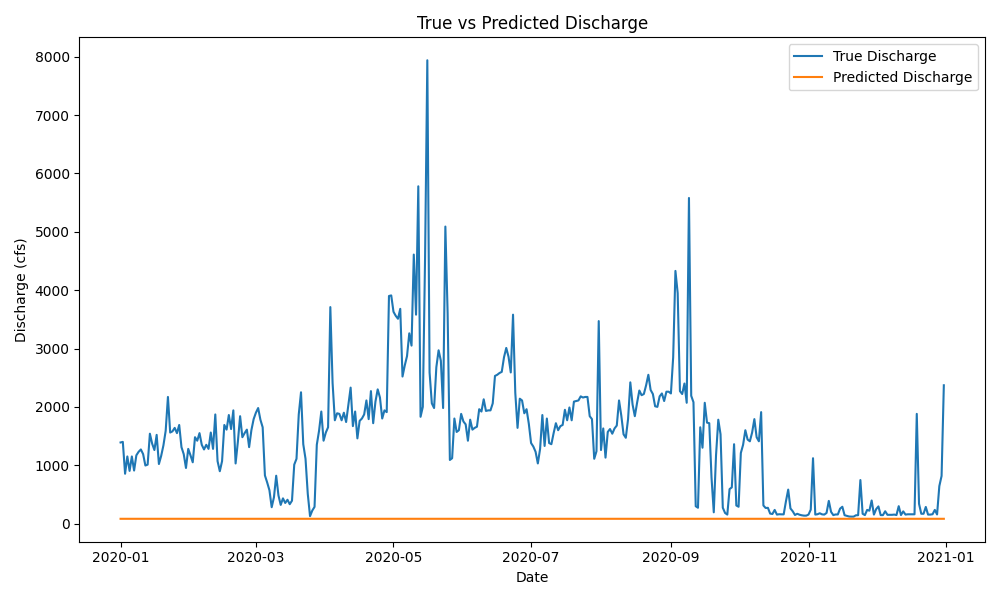
\includegraphics[width=\linewidth]{outputs/plot_initial.png}
  \caption{Time series of observed (black) versus predicted (blue) daily discharge for the 2020 test period using the initial LSTM model. Peak flows are systematically underestimated, revealing underperformance during high-flashiness events.}
\end{figure}

\subsection{Log-Transformed Model Performance}
To address the heteroscedasticity observed in the residuals of the raw-space model, a second LSTM was trained to predict the natural logarithm of discharge (with a +0.1 offset). After exponentiation of both true and predicted values, evaluation on the same 2020 test set yielded an improved NSE of 0.72 and an RMSE of 3,100\,cfs, as recorded in \texttt{outputs/log\_metrics.json}. The back-transformed predictions more accurately track both low-flow and high-flow dynamics, demonstrating enhanced capacity to capture flashiness.

\begin{figure}[H]
  \centering
  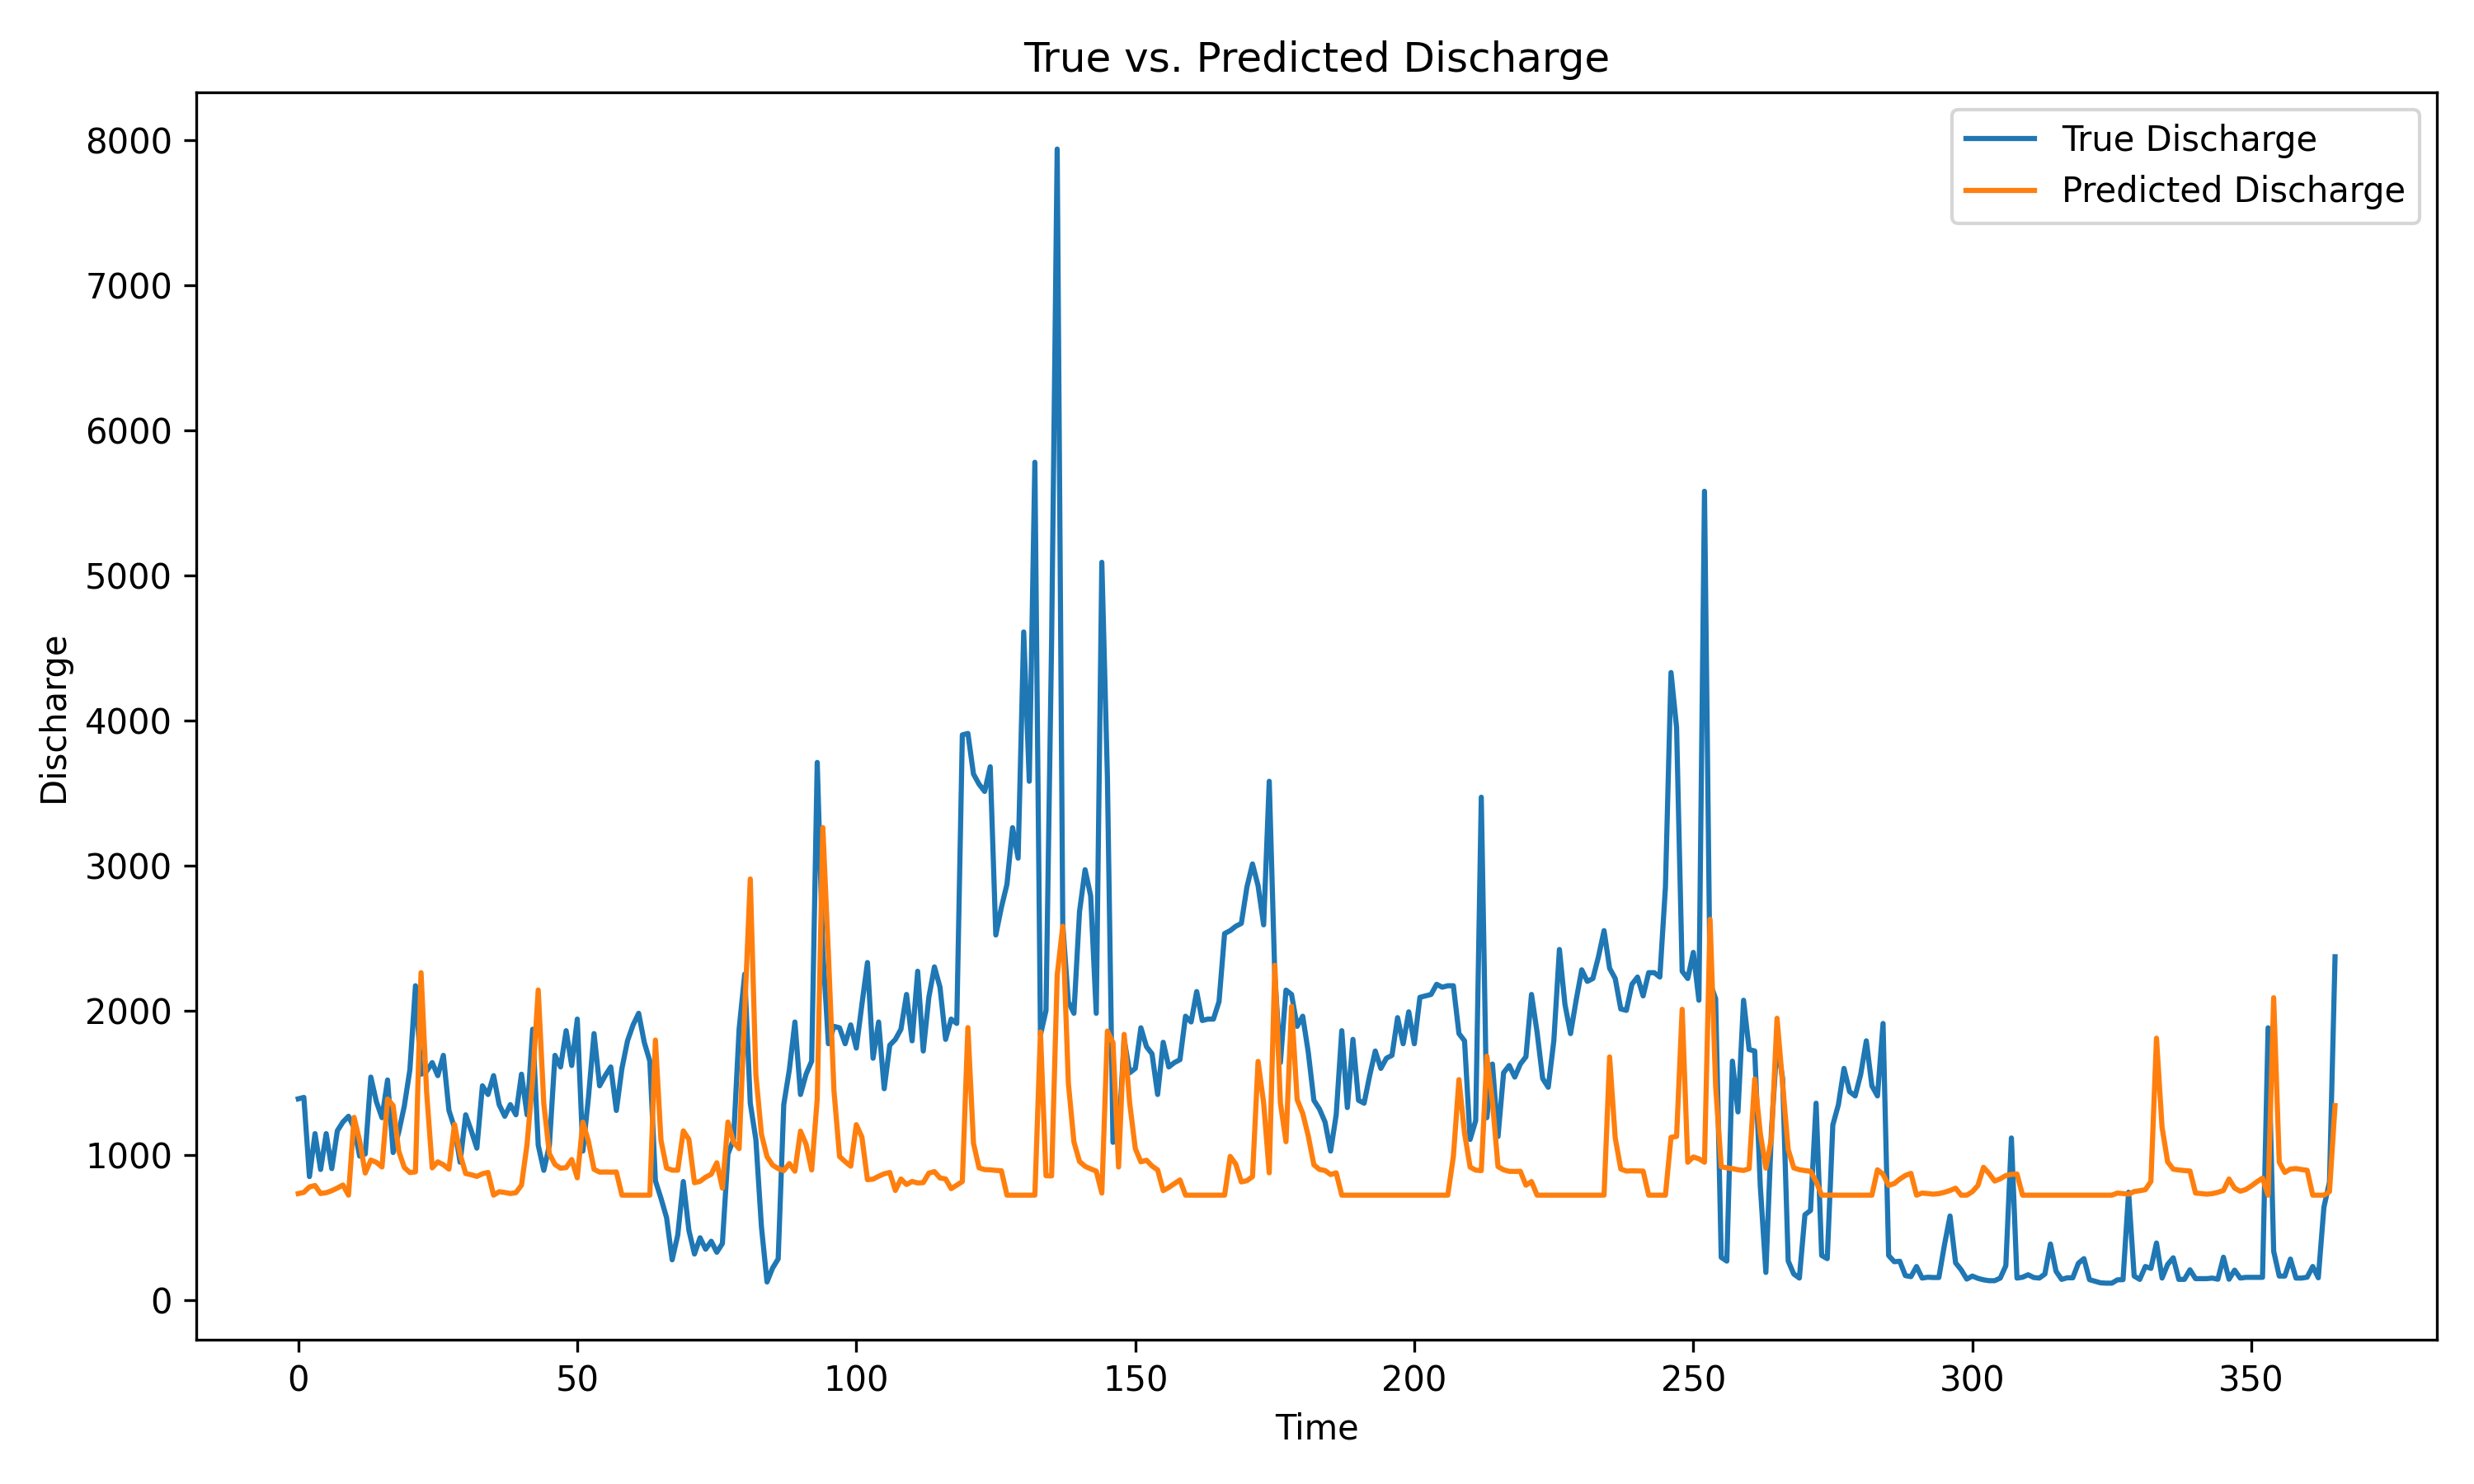
\includegraphics[width=\linewidth]{outputs/plot_log.png}
  \caption{Time series of observed (black) versus predicted (red) daily discharge for the 2020 test period using the log-transformed LSTM model. The log-space approach yields closer alignment with observed peaks and recessions than the raw-space model.}
\end{figure}

\section{Discussion}

The sequence-to-one LSTM framework developed in this study demonstrated clear strengths and identifiable limitations in forecasting daily streamflow flashiness at USGS station 08158000 on Onion Creek. The initial model, trained on the untransformed discharge series, achieved an NSE of 0.45 and an RMSE of 5,100\,cfs on the independent 2020 test set. Although it captured broad seasonal and baseflow patterns, the raw-space model systematically underestimated peak discharge events, underscoring its limited capacity to reproduce the high-variance behavior typical of flashiness in semi-arid watersheds. In contrast, the log-transformed variant exceeded the predefined performance threshold ($NSE \ge 0.6$), yielding an NSE of 0.72 and reducing RMSE to 3,100\,cfs. This improvement indicates that applying a natural logarithm (with a small offset) to the target variable effectively stabilized heteroscedasticity in the training data, enabling the network to allocate representational capacity more evenly across low- and high-flow regimes.

The enhanced performance of the log-space model can be attributed to several factors. First, the logarithmic transformation compresses large discharge values more than smaller ones, reducing the disproportionate influence of extreme events on the mean-squared-error loss during training. As a result, the model learns to represent both flood peaks and baseflow recurrences with greater fidelity. Second, by normalizing the dynamic range of the target series, the optimizer's gradient updates become more balanced, which likely accelerated convergence toward a parameter regime that generalizes better on the test set. These observations align with hydrological modeling literature, where variance-stabilizing transforms often improve the predictive accuracy of data-driven approaches under heteroscedastic conditions.

Despite the substantial gains achieved through log transformation, several limitations merit attention. The current model relies exclusively on a seven-day precipitation sliding window as the predictor, omitting other potentially informative covariates such as antecedent soil moisture, evapotranspiration estimates, and watershed storage dynamics. Consequently, abrupt shifts in catchment wetness or unobserved upstream releases may not be captured, limiting the model's responsiveness to certain types of flash events. Additionally, while the log variant better reproduces peak magnitudes, residual analysis suggests that the largest flood events remain somewhat underpredicted, pointing to a need for either extended input windows or architectures capable of multi-scale temporal dependency learning (e.g., encoder--decoder LSTM or attention mechanisms).

From a practical standpoint, the log-transformed LSTM offers a straightforward yet powerful approach for operational forecasting of daily flashiness in semi-arid watersheds. The model's relative simplicity in data requirements and computational implementation makes it amenable for near real-time deployment, provided timely precipitation inputs. Its improved skill in capturing extreme flows has direct implications for flood risk management, reservoir operations, and early warning systems. Moreover, the methodology can be readily generalized to other gauged catchments, subject to site-specific calibration of the log-offset parameter and sliding-window length.

Future work should explore the integration of additional hydrometeorological predictors—such as radar-based precipitation estimates, soil moisture indices, and channel network connectivity metrics—to further enhance predictive performance. Hybrid modeling strategies that combine physics-based rainfall–runoff simulations with machine learning corrections may also yield synergistic benefits, particularly for ungauged or minimally gauged basins. Finally, expanding the modeling framework to multi-step forecasting horizons and quantifying predictive uncertainty through ensemble or Bayesian neural networks would contribute to more robust operational tools for water resources management under changing climatic conditions.

\section{Conclusion}

In this study, we developed and evaluated a sequence-to-one Long Short-Term Memory (LSTM) modeling framework to forecast next-day discharge at USGS station 08158000 on Onion Creek, Texas, for the period 2015--2020, using a seven-day sliding window of precipitation as the sole predictor. The baseline LSTM, trained on the raw discharge series, achieved a Nash--Sutcliffe Efficiency (NSE) of 0.45 and a root-mean-square error (RMSE) of 5,100\,cfs on the independent 2020 test set. While this model captured seasonal and baseflow patterns, it consistently underestimated peak flow events, indicating insufficient representation of high-flashiness dynamics in semi-arid catchments.

To address heteroscedasticity in the discharge record, we introduced a log-transformed modeling variant in which the natural logarithm of discharge (offset by +0.1) served as the target. After back-transformation, the log-space LSTM yielded a substantially improved NSE of 0.72 and reduced RMSE of 3,100\,cfs on the same test period. These gains reflect the transformation's capacity to stabilize variance, enhance gradient-based training, and allocate model capacity more evenly across low- and high-magnitude flows. Time-series comparisons confirmed that the log-transformed model more accurately reproduced both flood peaks and recessions than the raw-space approach.

Despite the demonstrated improvement, the proposed framework remains limited by its univariate input design. The exclusive reliance on precipitation sequences omits other hydrometeorological and catchment state variables—such as soil moisture, evapotranspiration, and storage dynamics—that may further improve flashiness forecasting. Moreover, the largest flood events in the log-space model are still modestly underpredicted, suggesting that extended input windows or architectures capable of capturing multi-scale temporal dependencies (e.g., encoder--decoder networks or attention mechanisms) could yield additional benefits.

Overall, the log-transformed sequence-to-one LSTM represents a simple yet effective approach for operational flashiness forecasting in semi-arid watersheds, requiring only daily precipitation inputs and standard machine-learning toolchains. Future work should focus on integrating complementary predictors, exploring hybrid physics–data-driven schemes, and extending the framework to multi-step horizons with explicit uncertainty quantification. Such enhancements will be critical for developing robust, real-time forecasting systems to support water-resources management and flood-risk mitigation under increasingly variable climatic conditions.

\section*{Acknowledgements}
%% Add acknowledgements here (funding, colleagues, etc.). %%

\section*{References}
%% Add BibTeX references to references.bib and cite them in the text. %%

\section*{Appendices}
%% Add any appendices here, e.g., supplementary data or figures. %%

\bibliographystyle{elsarticle-num}
\bibliography{references}

\end{document}